\begin{frame}[allowframebreaks]{}
    \LARGE Normalizing Flow Models: \\[1.5ex] \textbf{Glow: Generative Flow}
\end{frame}

\begin{frame}[allowframebreaks]{Glow}
\textbf{Innovations:}

Introduced by Kingma and Dhariwal (2018), Glow incorporates:
\begin{itemize}
    \item \textbf{Invertible $1\times1$ convolutions} for channel mixing.
    \item \textbf{ActNorm layers} for data-dependent normalization.
    \item \textbf{Affine coupling layers} similar to RealNVP.
\end{itemize}

\textbf{Advantages:}
\begin{itemize}
    \item Improved expressiveness and stability.
    \item Enhanced performance in image generation tasks.
\end{itemize}
\framebreak
\textbf{Key Components:}
\begin{itemize}
    \item \textbf{ActNorm:} Applies per-channel affine transformation initialized with data statistics.
    \item \textbf{Invertible $1\times1$ Convolution:} Generalizes permutation operations, allowing learned channel mixing.
    \item \textbf{Affine Coupling Layers:} As in RealNVP, but integrated with the above components for greater flexibility.
\end{itemize}

\begin{figure}
    \centering
    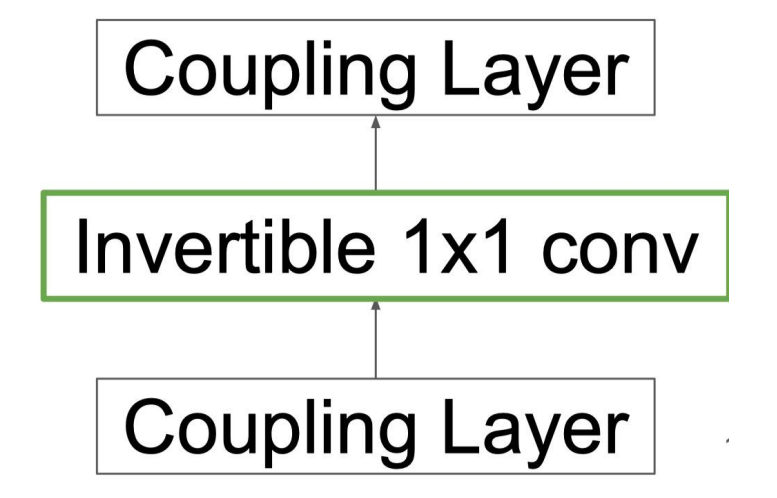
\includegraphics[height=0.4\textheight, width=\textwidth, keepaspectratio]{images/norm-flow/nfm_glow.png}
\end{figure}

\framebreak

\begin{figure}
    \centering
    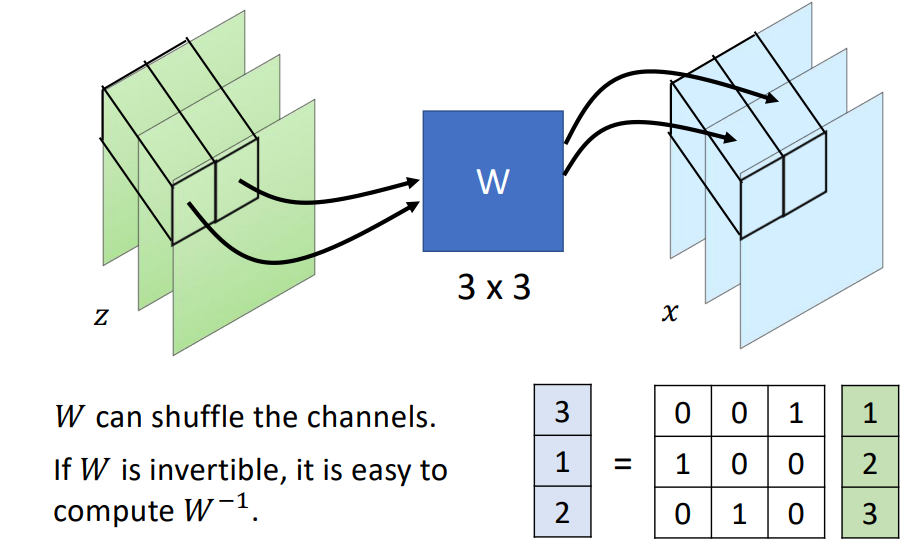
\includegraphics[height=0.9\textheight, width=\textwidth, keepaspectratio]{images/norm-flow/nfm_glow_1.png}
\end{figure}
\end{frame}

\begin{frame}[allowframebreaks]{Glow - Results}
\begin{figure}
    \centering
    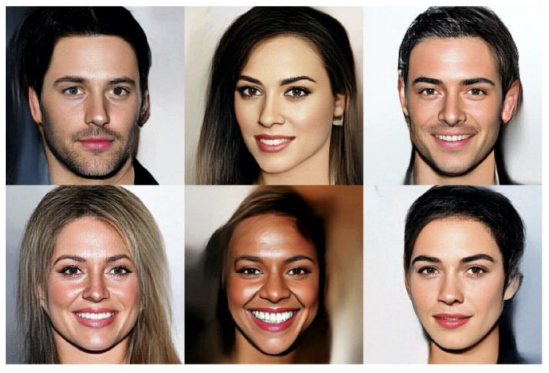
\includegraphics[height=0.8\textheight, width=\textwidth, keepaspectratio]{images/norm-flow/nfm_glow_results_1.png}
    \caption*{Glow generated samples}
\end{figure}

\framebreak

\begin{figure}
    \centering
    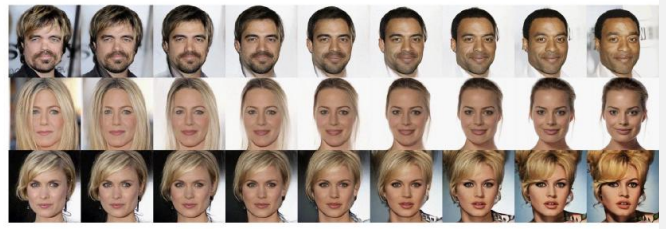
\includegraphics[height=0.8\textheight, width=\textwidth, keepaspectratio]{images/norm-flow/nfm_glow_results_2.png}
    \caption*{Linear interpolation in latent space between real images with Glow}
\end{figure}
\end{frame}